\documentclass[11pt]{article}
\usepackage[utf8]{inputenc}
\usepackage{blindtext}
\usepackage{setspace}
\usepackage{geometry}
\usepackage{graphicx}
\usepackage{mathtools}
\usepackage{unicode-math}
\usepackage{amssymb}
\usepackage{bm}
\usepackage[font={small}]{caption}
\geometry{a4paper, left=22mm,  top=22mm, bottom=22mm, right=22mm}
\usepackage[english]{babel}
\usepackage[sorting=none]{biblatex}
\usepackage{comment}
\addbibresource{bibliography.bib}


\begin{document}
\onehalfspacing
{
	\centering
	{\scshape\LARGE The University of Manchester \par}
	\vspace{1cm}
	{\scshape\Large BSc Dissertation\par}
	\vspace{1.5cm}
	{\huge\bfseries Correlation and attention in artificial intelligence\par}
	\vspace{2cm}
	{\Large Rutwik Mudholkar\\10327919 \par}
	\vspace{1cm}
	{\Large December 2020 \par}
	
	
}

\vspace{\fill}
\section*{Abstract}
Attention is an increasingly popular mechanism used in a wide range of neural architectures. It allows us to visualise their inner workings, a notoriously difficult task for an effective black box, and subsequently make better predictions for classification problems. Here we lay out the basic structure of a Convolution Neural Network optimised for Computer Vision image processing, and how an Attention Mechanism is implemented therein. We discuss different Attention Mechanisms, comparing their merits and use cases. We also discuss possible statistical theory underpinning the relation of Attention Mechanisms to measures of similarity and correlation to gain a deeper mathematical understanding of Attention.
\vspace{\fill}

\newpage
{\Large{\tableofcontents}}

\newpage
\setlength\parindent{0pt}
\section{Introduction}

Deep Learning, as a branch of Machine Learning, is closely related to a class of theories of brain development proposed by cognitive neuroscientists in the early 1990s \cite{utgoff}. Many proposed the neural networks used in deep learning models were analogous to learning dynamics in the brain. For instance, neural networks employing a hierarchy of layered filters in which each layer considers information from a prior layer, and then passes its output to other layers, is similar to the function of the cortex \cite{shrager}. The Convolutional Neural Network (CNN) in particular is a well-known deep learning architecture additionally inspired by the natural visual perception mechanism of living creatures. Computer vision based on CNNs has enabled people to accomplish what had been considered impossible in the past few centuries, such as face recognition, autonomous vehicles, self-service supermarkets, and intelligent medical treatment \cite{cnnintro}. \newline

Neuroscientists have long studied Attention as an important cognitive process. It is described as the ability of organisms to ‘select a subset of available information upon which to focus for enhanced processing and integration’ \cite{scholar}. The computational equivalent equips a neural network with the ability to focus on a subset of its inputs. The concept of ‘Attention’ has a long history in classical computer vision, where an Attention Mechanism selects relevant parts of the image for object recognition in cluttered scenes \cite{walther}. Paying attention to Attention is important for todays data heavy and computer intensive learning algorithms, as it provides essential cues for downstream Computer Vision models and frees up resources to focus on the most task-related parts of inputs \cite{borji}. In particular, understanding the mathematics of Attention Functions and how they measure the similarity, or correlation of relevant image parts may allow us to delve deeper into why they are so effective.\newline

Implementation of Attention can be done by analysing intermediate layers in a neural network pipeline. This dissertation will review different approaches to measuring correlations of these layers, and how they map to the different Attention Functions in CNNs.


\section{Artificial Neural Networks}
\subsection{Neurons}

Artificial Neural Networks (ANNs) are comprised of many interconnected computational nodes (referred to as neurons), which work in a distributed fashion to collectively learn from the input to optimise its final output \cite{chen}\cite{walczaka}. The basic unit of computation in a neural network is the neuron, often called a node or unit. It receives input from some other nodes, or from an external source and computes an output. \newline

The output Y from the neuron is computed as

\begin{figure}[htp]
    \centering
    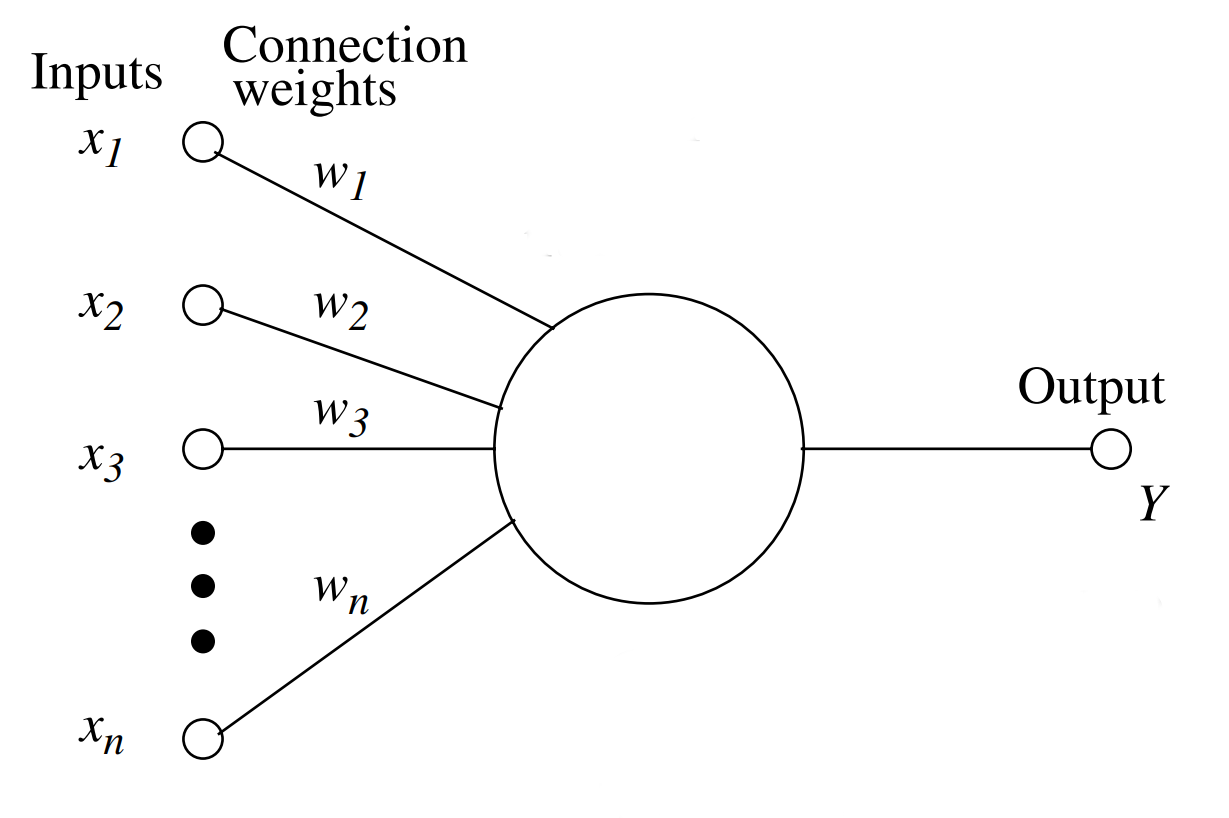
\includegraphics[width=9cm]{figures/neuron.png}
    \caption{ Diagrammatic representation of a neuron adapted from \cite{neuron}. It receives numerical inputs $x_1, x_2, ... x_n$ with respective weights $w_1, w_2, ... w_n$ and outputs $Y$.}
 \end{figure}   


\begin{equation}
Y = f(w_{1}x_{1}+w_{2}x_{2}+...+ w_{n}x_{n})
\end{equation} 

where ${x_i}$ are the numerical inputs, ${w_i}$ are the connection weights, and $f$ is non-linear and is called the Activation Function. The purpose of the Activation Function is to introduce non-linearity into the output of a neuron. This is important since real world data is non linear by nature, so we want our model to learn those representations \cite{baeldung}. 

\subsection{Feedforward Neural Networks}

Feedforward Neural Networks (FFFNNs) were the first and simplest type of ANNs devised \cite{ffnn}. They contain multiple neurons (also called nodes) arranged in layers. Nodes from adjacent layers have connections between them. All these connections have weights associated with them; given an input vector, they are the variables that determine what the output vector is. \newline

\begin{figure}[htp]
    \centering
    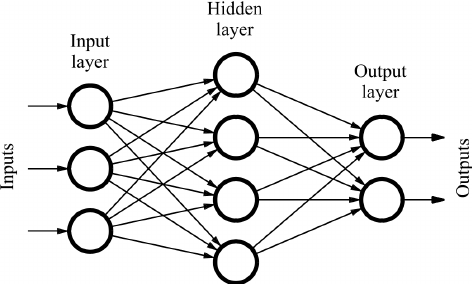
\includegraphics[width=9cm]{figures/ffnn2.png}
    \caption{Example of FFNN reproduced from \cite{ffnnpic}. It takes in 3 inputs and returns 1 of 2 outputs. $w^{h}_{ij}$ is the weight for a connection from the $i$th node in the $h$th layer, to the $j$th node in the next layer (weights not shown).}
 \end{figure}  
 
Figure 2 shows a simple example of a FFNN. The input nodes provide data to the network and are together referred to as the `Input Layer'. There is no computation at this stage; the data is simply piped to the hidden nodes. A collection of hidden nodes forms a `Hidden Layer'. While a FFNN will only have a single Input Layer and a single Output Layer, it can have zero or multiple Hidden Layers. The Hidden Layers perform computations and pass on their outputs to the next Hidden Layer. The final Hidden Layer transfers its outputs to the `Output Layer', which output the net result of the network. The information always moves in the forward direction, and there are no loops or cycles \cite{zell}. A FFNN with one or more Hidden Layers is called a Multi Layer Perceptron (MLP).\newline

Since we are interested in classification tasks using CNNs, we use an Activation Function in the Output Layer of the MLP such that the outputs are probabilities that sum to 1, such as a Softmax \cite{stanford}. Each output node is associated with some label e.g. ``dog'', ``cat'' etc. as classifications of an input e.g. an image of an animal. That way, given a vector of inputs $\bm{X} = (x_1, x_2, ... , x_i)$ that give a vector of outputs $\bm{Y} = (y_1, y_2, ... , y_j)$, the classification 

\begin{equation}
C = label(k),\ y_k = max(\bm{Y})
\end{equation}    

Since the initial weights are usually assigned randomly, The final output for an MLP has to be optimised through `learning'. The goal of learning is to assign correct weights for the connections. This can be done via `Backward Propagation of Errors', defined as `repeatedly adjusts the weights of the connections in the network so as to minimize a measure of the difference between the actual output vector of the net and the desired output vector' \cite{backprop}. This difference is the loss $L$ and is calculated via a loss function $L = f(\bm{Y}, \bm{\hat{Y}})$ where $\bm{\hat{Y}}$ is the desired output. Generally, $\hat{y_i} = \delta_{i,j}$ where j represents the desired label. In order to minimize $L$, it is propagated backward through the network to calculate the gradients 

\begin{equation}
\frac{\partial L}{\partial \bm{W}} = \{\frac{\partial L}{\partial w^{h}_{ij}}\}
\end{equation}

with respect to the weights. In a process analogous to numerically solving for the minimum of a curve, stochastic gradient descent is used to adjust the weights by 

\begin{equation}
w^{h}_{ij} \rightarrow w^{h}_{ij} - \epsilon\frac{\partial L}{\partial w^{h}_{ij}}.
\end{equation}

The choice of $L$ is contingent on the model type. For classification, Cross-entropy loss is preferred \cite{golik}. Backpropagation is usually used in conjunction with Whitening transformations to reduce Internal Covariate Shift \cite{batch}, the change in the distribution of network activations due to the change in network parameters during training. This can be achieved by standardising and scaling input data, such that the mean $\bm{\mu}_i$ of each input $\bm{X}_i$ equals 0, and that the covariances between each all the inputs are about the same \cite{lecun}. Whitening transformations can be affine such as the Mahalanobis Transformation:
\begin{equation}
\bm{z} = \bm{\Sigma}^{-1/2}(\bm{x}-\bm{\mu})
\end{equation}
where $\bm{\Sigma}, \bm{\mu}$ is the covariance matrix and mean vector for data vector $\bm{x}$. The univariate case for a scalar $x$ reduces to
\begin{equation}
z = \frac{x-\mu}{\sigma},
\end{equation}
which is the familiar form of a standardised normally distributed variable. These steps are taken in a traditional neural network to speed up the convergence of $L \rightarrow 0$, but for the case of an Attention based CNN, it also helps with finding an expression for Compatibility (Section 4).  A MLP is typically the last step of a CNN pipeline.


\section{Convolutional Neural Networks}

CNNs are a specialized type of neural network model designed for working with two-dimensional image data \cite{valueva}. LeNet was one of the very first and simplest CNNs \cite{culurciello} and is sufficient to explain the implementation of Attention.
\begin{figure}[htp]
    \centering
    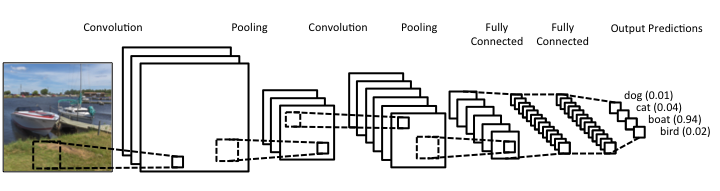
\includegraphics[width=17cm]{figures/cnn.png}
    \caption{Visualisation of the LeNET architecture reproduced from \cite{vogel}. The ReLU steps are not shown.}
 \end{figure}  
\subsection{High-Level Feature Extraction}
The three main levels for this stage are Convolutions, introducing Non Linearity, and Pooling. A Convolution (Fig. 3) is a linear operation involving an input tensor $\bm{I}$ and a Kernel tensor $\bm{K}$ to produce an 2D matrix $\bm{S}$ known as the `Feature Map', which can represented as

\begin{equation}
\bm{S}_{i, j}=\sum_{n}^{ }\sum_{x}^{ }\sum_{y}^{ }I_{i+x-1, j+y-1, n} \cdot \bm{K}_{x, y, n}.
\end{equation}

where $x, y$ are the dimensions of $\bm{K}$, $n$ is the depth of the tensor and the stride length is 1. In the case of $\bm{I}$ being an original colour image, it is split into 3 2D matrices using its colour channels (R,G,B), where each element is the channel pixel value. The matrices are concatenated to form a tensor of depth $n = 3$ . To retrieve each element of $\bm{S}$, $\bm{K}$ `strides' across $\bm{I}$ and performs the operation in Equation 4. $\bm{K}$ must be smaller than $\bm{I}$, and the specific size of $\bm{K}$ is decided prior based on certain factors \cite{sabyasachi}. The Convolution operation reduces matrix size since $\bm{K}$ cannot breach the boundary of $\bm{I}$, so if we want to ensure $\bm{S}$ and $\bm{I}$ have equal dimensionality, $\bm{I}$ is `padded' with additional row and columns to increase its size \cite{zhang2020dive}. Multiple Kernels can be used in one convolution layer to produces multiple Feature Maps, which are concatenated to form the new tensor. \newline

A nonlinear element wise operation is applied to the resulting Feature Map to introduce nonlinearlity into our CNN (see Section 2.1). One example is a Rectified Linear Unit (ReLU), given by 
\begin{equation}
\bm{S}_{i, j} \rightarrow max(\bm{S}_{i, j}, 0)
\end{equation}

Other non linear functions such as tanh or sigmoid can also be used \cite{chadha}. Spatial Pooling is then used to reduce the number of parameters and amount of computation in the network, hence controlling over-fitting while still retaining key features. In case of Max Pooling \cite{yamaguchi}, we define a spatial neighborhood (for example, a 2×2 window) and take the largest element from the rectified Feature Map within that window. The window $\bm{W}$ strides across $\bm{S}$ in a similar way to the Convolutional operation, however the stride length is now equal to the length of $\bm{W}$. Spatial Pooling can also be a Sum or Average. The Convolution, Nonlinear and Pooling steps can be successively performed multiple times, transforming $\bm{I} \rightarrow \{\bm{S}^1\} \rightarrow \{\bm{S}^2\} \rightarrow ... \rightarrow \{\bm{S}^L\}$ where $\{\bm{S}^l\}$ represents the set of Feature Maps at the $l$th layer of $L$ total layers along the CNN pipeline. 

\subsection{Training and Classification}
The training process for a CNN is similar to the Backpropagation of Errors and gradient descent model for a standard MLP (Section 2.2). The parameters learned are the connection weights for the Fully Connected MLP (FC) layers, and the values of the Kernel Filters. In practice, the set of Kernels that operate directly on the raw pixel values learn to extract low-level features, and sets operating on Feature Maps in subsequent layers learn to extract features that are combinations of lower-level features, such as lines and shapes. An example of a low-level Kernel Filter is that for for edge detection, which can take the form of

\begin{equation}
\bm{K} = \left[ \begin{matrix} -1 & -1 & -1 \\ -1 & 8 & -1 \\ -1 & -1 & -1 \end{matrix} \right]
\end{equation}

for the case $\bm{K} \in \mathbb{R}^{3\times 3}$. The resulting Feature Map would represent an image with sharper boundaries between objects and different colours, useful for extracting simple lines. This process continues until very deep layers are extracting faces, animals, and other complex objects \cite{chen2}\cite{layers2}. The final set of Feature Maps $\{S_n\}$ is turned into a 1D vector which is piped through a series of FC layers for classification. Figure 3 shows the original image being correctly classified as a `boat' with $P(boat) = 1$

\section{Attention}

\subsection{Inituition}

Extracting and choosing suitable features is crucial for image processing \cite{du}. However, this is challenging for images with complex backgrounds \cite{li}. One reason is due to the black box nature of CNNs; the visual reasoning they implement through their pipelines in solving problems remains largely inscrutable. A way to visualise and interpret the inner workings of CNNs, and thus extract useful data at intermediate layers throughout the process, is by the implementation of Attention, specifically finding the Attention Map. The Attention Map is a scalar matrix representing the relative importance of layer activations at different 2D spatial locations with respect to the target task \cite{simonyan1}. The Maps are used to exploit the effective spatial support of Feature Maps used by CNNs, based on the idea that there is benefit to identifying salient image regions and amplifying their influence, while likewise suppressing the irrelevant and potentially confusing information in other regions. Attention can be incorporated into any existing CNN architecture, including LeNet. \newline

One method to implement Attention-aware classification is by looking at the Compatibility between local feature vectors extracted at intermediate layers in the CNN, and the final global feature vector normally fed into the FC classification layers. Since this global feature vector represents salient higher-order visual concepts in different dimensions, this is achieved by encouraging our local feature vectors to learn similar mappings \cite{jetley}. Different kinds of class details are more easily accessible at different scales, so in order to facilitate the learning of diverse and complementary Attention-weighted features, layers are chosen based on different spatial resolutions. Rather than classify using solely this final feature vector like in a traditional CNN, we can restrict the classifier to instead use the intermediate local feature vectors, chosen and weighted by their Compatibility scores. The hyper-parameter here is the choice of Compatibility function, and is discussed further down.

\subsection{Implementation}

\begin{figure}[htp]
    \centering
    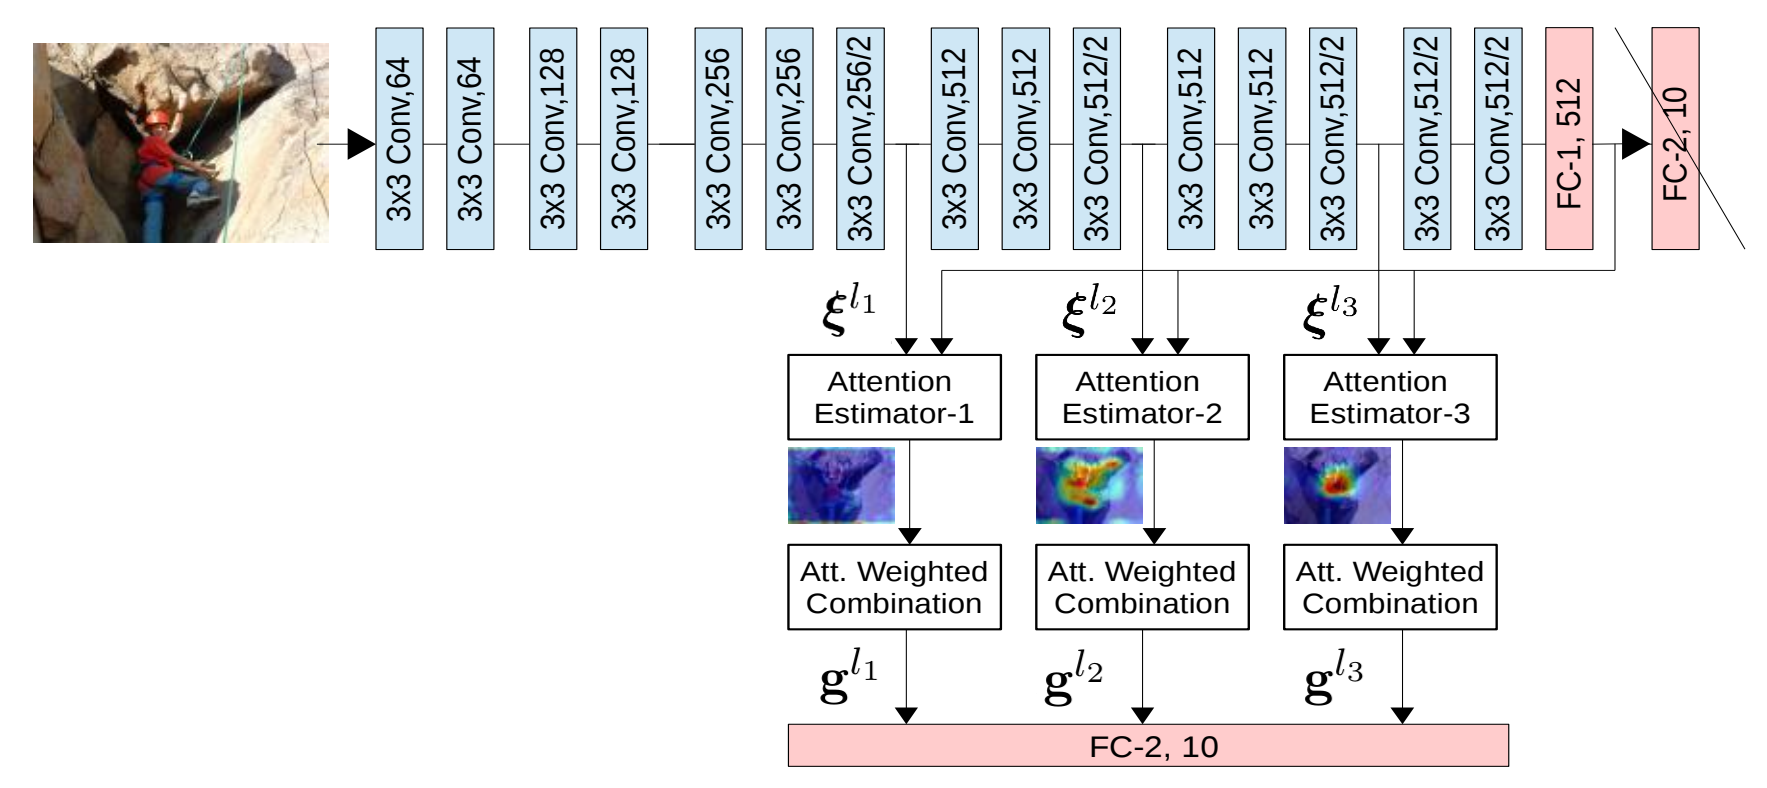
\includegraphics[width=17cm]{figures/cnnattention.png}
    \caption{Visualisation of Attention incorporated into a CNN architecture adapted from \cite{jetley}. Attention is introduced at 3 distinct layers, with the lowest level Attention Maps focusing on the surroundings (the rocks), intermediate level maps on object parts (harness and climbing equipment) and the highest level maps on the central object.}
 \end{figure}  

Consider the set of 2D Feature Maps $\{\bm{S}^l\}$ at layer $l$ as a 3D tensor $\bm{\xi}^{l}$ where $F_l$ is the depth, equal to the number of Feature Maps. $\bm{\xi}^{l} \equiv \{\bm{s}^{l}_{k}\}^{n}_{k=1}$, where each $\bm{s}^{l}_{k}$ represents the pixel-wise feature vector of length $F_l$ at the $k$th spatial location. Let $\bm{g} \in \mathbb{R}^{F_g}$ be the global feature vector extracted just before the final classification layer of a CNN. It has the entire input image as support and is output by the network’s series of convolutional and nonlinear layers. In this case $\bm{g}$ encodes global, discriminative, and relevant information about the objects of interest \cite{schlemper1}. We can now consider individual Attention Gates (AGs) at distinct intermediate layers to compute their Compatibility with $\bm{g}$. In order to produce the set of Compatibility scores \{${c^{l}_{k}}$\} at layer $l$, we use some Compatibility function $C(\bm{\xi}^{l}, \bm{g})$. In the case where $\bm{s}^{l}_{k}$ and $\bm{g}$ have different lengths, a learnable weight matrix $\bm{W}_g \in \mathbb{R}^{F_l \times F_g}$ can be used to match their lengths. \newline





For each $\bm{s}^{l}_{k}$, the AG then computes Attention Coefficients $A^l \equiv \{a^{l}_{k}\}^{n}_{k=1}$ where $a^{l}_{k} \in [0, 1]$, by normalising $\{c^{l}_{k}\}$ with a softmax function:
\begin{equation}
a^{l}_{k} = \frac{\exp(c^{l}_{k})}{\sum_{j}\exp(c^{l}_{j})}.
\end{equation}
The output of an AG at layer $l$ is given by a weighted sum $\bm{g}^l = \sum_{k}a^{l}_{k} \cdot \bm{s}^{l}_{k}$. The higher the $c^{l}_{k}$, the higher the $a^{l}_{k}$, meaning the corresponding $\bm{s}^{l}_{k}$ will be relatively weighted higher and have a stronger contribution to $\bm{g}^l$. The effect of an exponential rather than linear calculation greatly exaggerates small differences, ensuring $\bm{g}^l$ has minimal noise. Softmax also enforces $0 \leq a^{l}_{k} \leq 1\ \forall \in \{1 \dots n\}$ and $\sum_i a_i = 1$, so the combination of feature vectors is convex. This ensures that features at different spatial locations must effectively compete against one another for their share of the Attention Map. We can now constrain our final FC inputs to a new set $\{\bm{g}^l\}$ from all AGs, forcing our network to learn the most salient features that contribute to the class. Since the Attention Mechanism has access to the entire image, we call it `Soft' Attention, since the learned alignment weights $a^{l}_{k}$ are placed `softly' over all patches in the source image. This makes the image smooth and differentiable, but computationally expensive when the source image is large. `Hard' Attention \cite{luong} on the other hand only selects one patch of the image to attend to at a time, making it cheaper, but requiring more complicated techniques such as variance reduction or reinforcement learning to train. 

\section{Compatibility and Correlation}

$C(\bm{\xi}^{l}, \bm{g})$ is one of the most important hyper-parameters that differs in literature based on various input image attributes. The two groups of Compatibility functions used in computer vision based CNNs are Multiplicative and Additive Compatibility (MC, AC respectively). However, how these exactly translate to mathematical strengths of relation and similar mappings is scarcely studied in literature. The method by which we vary the Attention Mechanism will be solely varying $C(\bm{\xi}^{l}, \bm{g})$, since it is the only step which compares the two vectors.

\subsection{Multiplicative Compatibility}

MC has the general form
\begin{equation}
c^{l}_{k} = \bm{s}^{l}_{k} \cdot \bm{g}
\end{equation}
as used in \cite{jetley}. We could interpret this as the unnormalized form of cosine similarity, which measures the degree of alignment of two vectors. We can see it resembles Pearsons correlation coefficient (PCC) \cite{pearson}, which uses the normalised form of the co-variance, which itself is a dot product between the deviations of two raw data sets from their mean. MC is a raw dot product, however. Consider 3 channel colour images with pixel values ranging between 0 and 255, with feature vectors $\bm{s}^{l}_{k}$ having $\bm{\mu}_i > \bm{0}$ and covariance $\bm{\Sigma}$. The more $\bm{\mu}_i > 0$ strays from 0, the less MC may represent correlation. This issue is noticeably amplified in the case $\bm{\mu}_i \neq \bm{\mu}_j, \delta_{ij} = 0$, where $\bm{s}^{l}_{k}$ with higher means will naturally give higher dot products, regardless of correlation. This issue can be resolved by the zero centering normalisation of input data done by whitening of the feature vectors at each layer during backpropagation (see Section 2.2). In this case $\bm{\mu} = \bm{0}$, reducing MC to PCC. We can therefore see that MC represents mapping similarity via correlation. \newline

\begin{figure}[htp]
    \centering
    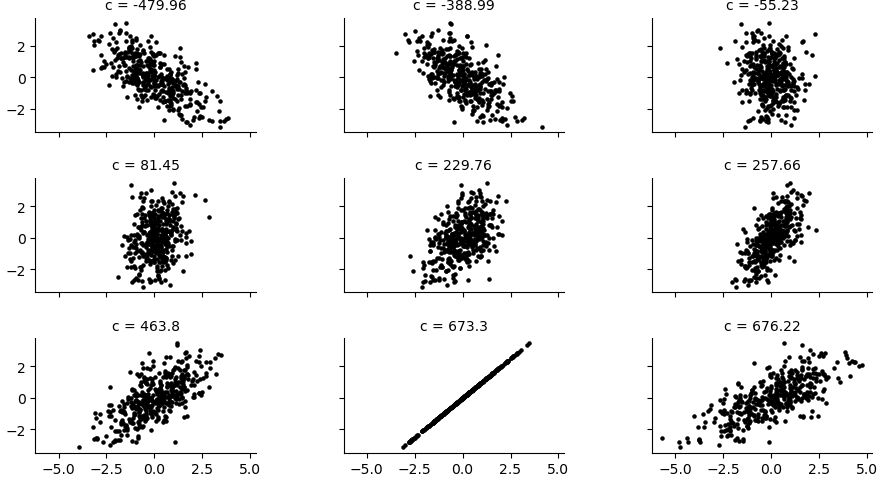
\includegraphics[width=15cm]{figures/cnnfig3.png}
    \caption{Plots 1 to 9 of vectors $\{\bm{v}\} \sim N(\bm{0}, \bm{\Sigma}), |\{\bm{v}\}| = 9$ against a vector $\bm{v}_k \in \{\bm{v}\}, k=5$ with their Compatibility scores $c$ calculated using Equation 11. Plot 8 is vector $\bm{v}_k$ against itself}
 \end{figure}
 
From Figure 5 we can see this relation. $\bm{\mu} = \bm{0}$, and $\bm{\Sigma}$ is randomly generated and multiplied by a scalar $\epsilon \sim 10^{-3}$ to approximate the whitening covariance similarity condition. Here, $c$ increases proportionally to the perceived strength of positive correlation between the two vectors. Inserting the set of Compatibility scores into Equation 8 will yield exponentially increasingly larger attention Coefficients for plots 4 to 9, and yield effectively 0 for plots 1 to 3. The Attention Coefficient ratio between plots 8 and 9 is $e^{676.22}/e^{673.3} \sim 10^{1}$, and between 7 and 8 is $e^{673.3}/e^{463.8} \sim 10^{90}$, a huge magnitudinal difference that leaves only 8 and 9 contributing to $\bm{g}^l$. While still Soft Attention, it borders on Hard Attention, and will produce a sharp Attention Map. We see a discrepancy with plots 8 and 9, where a noticeably lower correlation generates a higher Compatibility score. This can be explained by edge conditions, wherein the range of pixel values deviates further from the mean in plot 9, likely due to the small fluctuations in $\bm{\Sigma}$. This can be resolved by restricting the range or further equalising the co-variances through back-propagation. It may also be minimized by only extracting Feature Maps at deep layers, where the numerous Convolutional filters beforehand have removed pixel noise and made them sparse. Sparse Feature Maps have many pixels close or equal to 0 (`deactivated') while the others have high activations, a natural consequence to extracting salient features. This would result in the data within $\bm{s}^{l}_{k}$ resembling a more discrete distribution. In this case, only mutually activated pixel vector indices would contribute. Another reason to extract at deeper layers is that the effective filters operating over image patches in the layers represent relatively `mature’ features with respect to the classification goal, so will tend to simply be closer to $\bm{g}$. Scaled MC          

\begin{equation}
c^{l}_{k} = \frac{\bm{s}^{l}_{k} \cdot \bm{g}}{\sqrt{d_k}}
\end{equation}

used in \cite{vaswani} may be modified to resolve any scaling issues brought up by down-sampling from pooling layers, which create local feature vectors of different dimensions. Here $\sqrt{d_k}$ represents the dimension of a key for natural language processing in Recurrent Neural Networks (RNNs), and the scaling counteracts the fact that the dot product grows with $\sqrt{d_k}$. Another scaled version is the cosine similarity

\begin{equation}
c^{l}_{k} = cosine[\bm{s}^{l}_{k}, \bm{g}] = \frac{\bm{s}^{l}_{k} \cdot \bm{g}}{||\bm{s}^{l}_{k}|| \cdot ||\bm{g}||}
\end{equation}

as used in \cite{graves}, which measures the cosine angle between the two vectors. This by definition is a measure of alignment, where the correlation can be interpreted as how parallel the two vectors are. The scaling factor of the magnitudes ensures high-valued feature vectors are not over-represented. This model is also usually used for RNNs. \newline

\begin{figure}[htp]
    \centering
    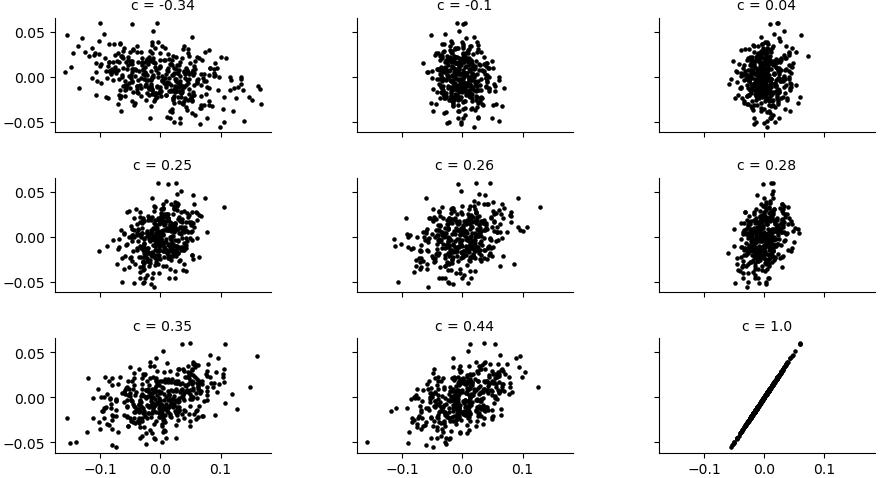
\includegraphics[width=15cm]{spearman.png}
    \caption{Plots 1 to 9 of a new set of vectors $\{\bm{v}\} \sim N(\bm{0}, \bm{\Sigma}), |\{\bm{v}\}| = 9$ against a vector $\bm{v}_k \in \{\bm{v}\}, k=5$ with their Compatibility scores $c$ calculated using Equation 14. Plot 9 is vector $\bm{v}_k$ against itself}
 \end{figure}
 
The Spearmans rank correlation coefficient (SRCC) is another widely used measure of correlation, and is defined as PCC between the rank variables \cite{myers}. While PCC assesses strictly linear relationships, SRCC assesses monotonic relationships (whether linear or not). A monotonic function preserves or reverses the order between two ordered sets, hence the term `rank'. If there are no repeated data values, a perfect SRCC of $+1$ or $-1$ occurs when each of the variables is a perfect monotone function of the other. Not only is SRCC appropriate for both continuous and discrete variables \cite{lehman}, it will likely better fit the often nonlinear feature vectors as long as they are monotonic in nature. As a Compatibility function, we use the discrete form 
 
\begin{equation}
c^{l}_{k} = 1 - \frac{6\sum^{n}_1 d_{i}^{2}}{n(n^{2}-1)}
\end{equation}

where $n$ is the number of ranks, given by the integer length of the feature vectors. We are assuming their dimensionalities have been scaled to equal each other. $d_{i}$ is difference between the element ranks of the two vectors at index $i$. SRCC Compatibility is trivially a measure of correlation. Figure 6 shows an improvement over Figure 5, correctly ordering the plots by their strength of correlation, and fixing the range issue. Since $c^{l}_{k} \in [-1,1]$, the exponential weighting will not be as harsh. The maximum magnitudinal difference is only $e^1/e^{-1} \sim 10^1$, thus will yield much softer Attention than general MC above. This could be beneficial for noisy data, where salient regions have broader distributions. SRCC Compatibility is, however, absent in Attention literature. This is likely due to the Attention being, in fact, too soft. Exponential weighting on Feature Maps with hundreds of feature vectors will not be sufficient to highlight salient regions at all; $a^{l}_{k}$ for highly correlated $\bm{s}^{l}_{k}, \bm{g}$ will quickly be drowned out, and produce homogeneous Attention Maps. This could fixed by multiplying all $c^{l}_{k}$ by a constant scalar $r>1$ to extend the range to $[-r,r]$. This adds a data-contingent continuous hyperparameter however, which is unideal for creating a universal CNN that requires no human adjustment to achieve optimality. Figure 7 highlights the stark difference in softness between the SRCC and General MC Attention Maps, with just 9 data points.

\begin{figure}[htp]
    \centering
    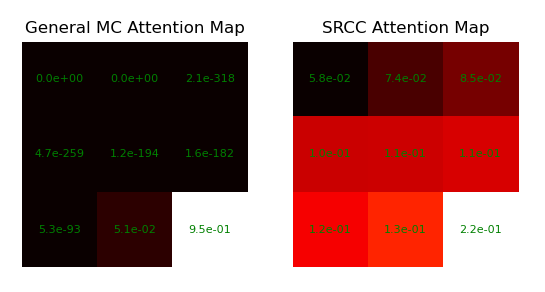
\includegraphics[width=12cm]{figures/attentionmap.png}
    \caption{Attention Heat Maps representing the Attention Coefficients of plots 1-9 from Figures 5 (General MC) and 6 (SRCC), calculated using Equation 10. the higher the Attention Coefficient, the lighter the colour.}
 \end{figure}
\vspace{-0.5cm}
\subsection{Additive Compatibility}

The alignment model from \cite{bahdanau} can be re-purposed as an AC function given by

\begin{equation}
c^{l}_{k} = \bm{\Psi} \cdot (\bm{s}^{l}_{k} + \bm{g})
\end{equation}

where $\bm{\Psi} \in \mathbb{R}^{F_l}$ is a learnable parameter, and can be interpreted as learning the universal set of features relevant to the object categories in the dataset. Since free parameters exist between the local and the global image descriptors in a CNN pipeline, we can generalise concatenation of the two descriptors to an addition operation. This allows us to limit the parameters of the Compatibility function. We then learn a single fully connected mapping from the resultant descriptor to the Compatibility scores. In order to introduce more variability for maximum alignment, this can be extended to a more general linear additive model given by 

\begin{equation}
c^{l}_{k} = \bm{\Psi}act(\bm{W_s}\bm{s}^{l}_{k} + \bm{W_g}\bm{g} + \bm{b_g}) + b_\Psi
\end{equation}

as used in \cite{schlemper1}, where $\bm{W_s} \in \mathbb{R}^{F_{x} \times F_{l}}, \bm{W_g} \in \mathbb{R}^{F_{x} \times F_{g}}, \bm{\Psi} \in \mathbb{R}^{C_x}$ and bias terms $b_\Psi \in \mathbb{R}, \bm{b_g} \in \mathbb{R}^{C_x}$. $act$ is a nonlinear activation function, such as ReLU. The benefit of the generalised approach is that introducing $\bm{W_s}$ allows the deeper fine-scale layers to focus less on generating a signal that is compatible to $\bm{g}$, which helps it focus on learning the discriminant, diverse features. By also introducing $\bm{W_g}$ and $act$, the network is allowed to learn nonlinear relationships between the vectors, which is more expressive (see Section 2.1). This is especially important in applications where images have an inherently higher noise to signal ratio, such as Magnetic Resonance Imaging (MRI), where the region of interest is often highly non-homogeneous. A strictly linear AC model may be too sensitive to such fluctuation. For instance, consider the edge detection Kernel $\bm{K}$ from Equation 9 incorporated in a Convolutional layer to help extract boundaries of brain regions in MRI scans. In a noisy scan, the boundary may be blurred and melted into its surroundings, thus $\bm{K}$ will fail to fully highlight the boundary edge. MC will interpret this as a non-salient region, however a nonlinear AC model could learn to identify the resulting underlying distribution of pixel values due to $\bm{K}$ as salient. AC seems appropriate in most if not all case, but is far more computationally expensive than standard MC, since it incorporates an additional learning component. It should therefore be used primarily for low resolution, noisy data like MRIs, while MC is preferable for dense, multi-channel images. \newline

This general model doesn't resemble any common existing measures of correlation. However, it does resemble the function of a single neuron, since it contains a linear function of weights and inputs, followed by a non-linearity. Since the inputs themselves are vectors, it can be interpreted as a single-layer MLP, where the weight matrices are learned via back-propagation. In this case, the Compatibility of the local and global vector isn't derived from a strict, constant method, but instead learned by analysing the final output. Since an arbitrarily large MLP is a universal function approximator \cite{sifaoui}, a trained single-layer MLP as an AC can be interpreted as an alignment, or dataset specific correlation approximator. 

\subsection{Significance}
There is a mathematical significance of Compatibility representing a measure of correlation rather than pure equivalency. Consider an image piped through a trained Attention-based CNN. Now consider the same image, but with a higher contrast, or exposure, or a similar transformation that changes all the pixel values, but retains features. The raw equivalence between the original and altered will be drastic, and taking a matrix difference will yield a high deviation. However, analysing the pixel mapping will yield a constant relation that can described as a correlation. For instance, every pixel may be multiplied a scalar $k$, or blurred with a Kernel matrix. Therefore, if two images are considered to be correlated rather than equivalent, we can say they contain the same features. $C(\bm{\xi}^{l}, \bm{g})$ should therefore yield similar Compatibility scores, and thus output the same $\hat{y_i}$. Another implication is that for images with a high signal to noise ratio, where we can look toward other commonly used multiplicative correlation measures to measure our Compatibility; the total number is theoretically infinite. \newline

Moving past pure statistics, the biological significance cannot be understated. Attention is the next logical step in bridging the gap between Artificial Intelligence and Human Intelligence. Understanding what it measures can give us insight into what `measure' our brain uses to continuously and subconsciously identify salient regions in what it sees.


\section{Conclusion}
As society becomes more automated, the demand for highly efficient Artificial Intelligence algorithms to process vast amounts of data is ever increasing. CNNs for Computer Vision are just one of many. The implementation of Attention increases efficiency by identifying salient regions of images prior to classification, bearing a striking semblance to human vision. Analysis shows all forms of Multiplicative Compatibility can be interpreted as measures of correlation. Additive Compatibility is a learned process that resembles no existing correlation measure, but through training can be interpreted as learning a data specific alignment, or correlation approximator. MC measure are sensitive to noise, different measures produce vastly different results, but are computationally cheap. AC takes a universal form, handles noisy data well, but is computationally expensive.

\newpage
\printbibliography
\end{document}

\begin{comment}

TODO

Title graphs

\end{comment}
